\documentclass{vivid_layout}

% \makeprint is for printing and trimming on paper, w/crop marks.
% \makeprint

%% Required to build cover page
\title{\fontsize{32pt}{15pt}\selectfont How to Architect and Build}{\fontsize{30.2pt}{15pt}\selectfont Highly Observable Systems}
\date{\color{white} \today{} \textbullet{} Revision 2}
\cover{architecture-monitoring/cover}

%% Required to build "Meet the Author"
\author{Baron Schwartz}{img/baron}

%% Required image for "About VividCortex"
\aboutvc{img/presenter}
\nopagebreak
%% Required resource info
\resourceleft%
	{Practical Scalability Analysis with the Universal Scalability Law}
	{The Universal Scalability Law models how systems perform as they grow. This
	52-page book shows how to use it for practical
	purposes such as capacity planning.}
	{img/scalability}
	{https://www.vividcortex.com/resources/universal-scalability-law/}
\resourceright%
	{Case Study: Tradesy}
	{After deploying VividCortex, Tradesy reported
	``We were able to bring maximum CPU utilization spikes down from 80\% to
	10\%. VividCortex is incredibly straightforward---it's the best MySQL tool I’ve ever used to monitor and analyze databases.''}
	{img/tradesy-thumbnail}
	{https://www.vividcortex.com/resources/tradesy/}

\begin{document}
\maketitle		% Build the cover page
\begin{bio}		% Biographical info for "Meet the Author"
Baron is a performance and scalability expert who participates in various
database, opensource, and distributed systems communities. He has helped build
and scale many large, high-traffic services for Fortune 1000 clients. He has
written several books, including O'Reilly's best-selling High Performance MySQL.
Baron has a CS degree from the University of Virginia.
\end{bio}
\tableofcontents	% Build the table of contents

\section{Introduction}

Is your application easy to monitor in production? Many are, but
sadly, some applications are designed with observability as an afterthought.
Consequences include problems such as:

\begin{itemize}
\item It's cost-prohibitive to monitor and troubleshoot the app in production.
\item Developers don't know how the app works, so changes are riskier and more costly.
\item No existing systems can monitor the app, so you are forced to develop
something custom.
\item The app's instrumentation is lacking, incompatible with popular monitoring
systems, or impossible to correlate with other metrics.
\item Adding instrumentation is impossible, limiting visibility.
\item People, processes, and systems related to monitoring and observability become
a productivity bottleneck, leading to shipping code more slowly with more frequent
and costly problems.
\end{itemize}

Observability is one of the most important factors of building and running services
successfully at scale. It's best to build it in from the start, just
like backups, security, auditability, and the like. In this way, you can make tradeoffs
and plan for the future proactively, instead of accidentally.

This ebook collects the experience of a variety of experienced architects and
combines it with what customers have taught us about observability at
VividCortex. My hope is that you will be able to apply the best practices in
this book to avoid pitfalls later, and create a highly observable
application, so you can get excellent visibility and troubleshooting ability with
minimal cost and effort. 

My personal experience is rooted in database observability, where I've spent the last 15
years of my professional career. What I've learned about database performance is
entirely a result of understanding database observability. This is a special case
of observability, with more challenges and constraints that make it harder than the general case. But I've built and run a variety of systems at scale, not just databases, and I hope you'll find my experiences relevant to what you're doing too.

\section{What is Observability?}

Over the last several years, observability has emerged into the popular consciousness
of software engineers, SREs, and DevOps practitioners as one of the key attributes
of well-built systems. But what is observability? In some circles, it's old wine in a
new skin: just a faddish name for monitoring.

I don't see it that way at all. Observability is a property of an application, and monitoring is an activity one does; observability is a noun and monitoring is a verb. There's a formal definition of observability from control theory, but it really is pretty simple: an application or system is observable if you can understand its inner workings by measuring its external behaviors. These behaviors are exposed through telemetry, which is the data emitted from instrumentation.

In contrast, monitoring is the activity of analyzing the system's telemetry, and testing whether it's functioning correctly. Diagnostics is the process of determining what’s wrong with a system, and also relies on observability. In other words, monitoring tells you whether a system is working; observability helps you answer why.

\section{What Should You Monitor?}

Observability is the foundation for monitoring, but it doesn't automatically make monitoring easy.

One of the most common questions people ask when installing and configuring
monitoring systems is ``what should I monitor?'' This is an excellent guiding
question to use for discussing the goals and characteristics of a highly observable application. Any critical system typically tends to emit a lot of telemetry. Databases, for example, often have hundreds of status counters that can become metrics in a traditional monitoring system. How can you make sense of such complexity? What should you pay attention to? What's core and what's secondary?

A formal framework really helps here. Without getting into the underlying theory, the framework that I've developed over many years (standing on the shoulders of giants) focuses on holistic observability in two directions: \emph{external quality of service} and \emph{internal sufficiency of resources}. Anchoring to these two perspectives, there are simple methodologies, which help reduce the complexity and make it manageable. As a result, you'll be able to \emph{measure what you should, not what you can}.

Externally, you should measure whether the application or system is providing good quality of service to its customers. That is easy to understand if you restate it in a customer-centric viewpoint: customers (or users) are asking the system to do work for them; good quality of service is delivered when they get correct, fast answers. Thus, external quality of service is about measuring \emph{requests}.

High-traffic services handle too many requests to measure individually, so you'll need aggregate measures that help you understand the population as a whole. The four golden signals of workload quality-of-service are:

\begin{description}
	\item[Concurrency] Concurrency is the total number of requests in process, either at an instant in time or over a duration. It's a dimensionless measure of load, which is another way of saying how much work the system is doing, in total. This is the single best measure of service demand placed on the service. Concurrency is the underlying metric of load metrics you're familiar with, such as load average and backlog.
	\item[Error Rate] The error rate is the proportion of requests that aren't successful. Customers care about getting a successful, correct reply to their request.
	\item[Latency] Second only to a successful response is a fast one. Latency is the measure of how long it takes for the customer or user to get their reply back, in units of seconds per request. It's best measured end-to-end. You can aggregate lots of individual requests' latencies over an interval; either by averaging them (less desirable) or by producing long-tail metrics such as the 99th percentile latency (better).
	\item[Throughput] This is the rate of requests, expressed as requests per second over a time interval. In combination with latency and concurrency, it answers questions such as whether the service is getting slower, or just more heavily loaded; whether it's gotten stuck, or just stopped being sent traffic from upstream.
\end{description}

These four metrics together form the CELT acronym that we use at VividCortex to characterize workload quality-of-service from the end-user's point of view. These four are necessary and sufficient for detecting and explaining the nature of (but not always the causes of) every possible performance problem a system can experience. In other words, if these four golden signals don't show a problem, there isn't a problem (from the customer's point of view).

You might have heard of the ``RED Method." CELT is essentially the same but uses standard terminology from performance theory, and adds the critical dimension of Concurrency (e.g. load, service demand). The RED metrics (rate, errors, duration) map to three of the four CELT metrics (throughput, errors, latency). What RED and CELT share in common is a belief that system performance has to be defined from the perspective of the customer or end user. Nobody whose requests are timing out and failing cares about how many nines of availability the server has or how busy its CPU is. As Charity Majors says, nines don't matter if users aren't happy.

Is the external quality-of-service enough to measure? No, because it doesn't explain \emph{why} things are slow for customers. For that, you do need to measure the system or server itself. In particular, you need to measure the four key resources (CPU, memory, storage, and network) and for each of these, you need to measure three golden signals: Utilization, Saturation, and Errors. These three constitute \href{http://www.brendangregg.com/usemethod.html}{Brendan Gregg's USE method}, which is extremely helpful for navigating complex systems and determining whether they're the bottleneck. In addition, many systems have their own custom-built resources, such as thread pools or queues, which you should measure the same way.

If you put these two together---the workload and its quality of service, plus the system's resources and their sufficiency to service the workload---you have a compact set of things to measure and monitor that's typically a lot smaller than the totality of what you could spend your time and effort examining.

These signals---CELT plus USE---apply universally to all systems and software. Again, they're based on formal performance theory, bringing together the totality of things like queueing theory, Little's Law, and more. These seven golden signals are necessary and sufficient to understand your custom software as well as canned ``off-the-shelf" software such as your favorite database.

In databases, in particular, the most important thing to measure is queries (or
statements, or requests, or similar).  Queries are the database's unit of work; measuring all of the database's queries is measuring its workload. Because databases are hard-to-monitor, it turns out that query monitoring is hard no matter how you do it, but later in this book I'll spend some time discussing how to do it the best you can.

Whew! That's a lot to think about.
That's why this book's focus is much more on \emph{guidelines} to help you structure the world and divide-and-conquer observability problems, than on 
lists of metrics or recipes and the like. As we dive deep, you'll see
more examples that can illustrate specific cases and provide
principles you can apply broadly.

\section{Observability Tradeoffs}

Monitoring, like any other engineering activity, is a set of decisions and
tradeoffs among many competing priorities. In this
section, I'll discuss some of those tradeoffs, in hopes of helping you make
choices that will lead to better outcomes.

Here are a few of the most important tradeoffs I've seen:

\begin{description}

\item[Developer Friendliness vs. Operability] If you build your application to be
developer friendly, but ignore how it runs in production, you'll
likely end up with an app that is harder to deploy, operate, and monitor. These need not
be mutually exclusive goals---but if operability is an afterthought, you might
make many decisions that \emph{do} preclude choices later.

\item[Your Process vs. Monitoring Software] All software, including monitoring
systems, expresses a worldview and workflow. When these don't match your own,
you have to prioritize: do you adopt your systems and practices to fit into
the monitoring software, or do you require it to support your workflow? Do you build
the observability you need, or do you just measure what you can with your monitoring software?

\item[Cost vs. Observability] In many cases, the more observable a system is, the
more expensive it is to monitor. This follows rather directly from the amount of
monitoring data you can collect from the system and the granularity at which you
collect it. Monitoring can be expensive if you collect a lot of data, but it can
pay off. I've been told that Netflix's monitoring systems are a double-digit
percentage of their overall operating budget. Netflix has even been described as
a monitoring company that happens to stream movies. At the same time, Netflix's
revenue per employee is one of the highest among publicly traded companies.
Coincidence? You decide.

As another example, I know of many companies migrating from Oracle to PostgreSQL
for cost reasons. The licensing cost is certainly much lower, but there's 
no comparison between the amount of observability Oracle provides and what you can
get in PostgreSQL. Is the compromise worth it? That's a decision you have to
make.

\item[Isolated Services vs. Monoliths] Microservices architectures increasingly popular. We're big fans of some of the principles of microservices at
VividCortex. But we've seen many customers struggle with the
implications of monitoring microservices, especially when taken to extremes.
Many small pieces create many sources of metrics, which means many metrics (high cardinality), which
makes sophisticated and cost-effective monitoring systems a must. Likewise, lots of metrics leads
to high cost, which I addressed in the previous point (cost versus
observability).

This point also applies to another current hot topic, containerization. If you
ship tons of Docker containers and run lots of them in production, you have that
many more things to monitor. Likewise, whether you isolate every different
workload onto different databases, or you have some databases that handle
multiple workloads---or even whether you want to run a few big powerful database
servers versus lots and lots of small cheap ones.

Cost and scale of telemetry is not a small consideration. Depending on the monitoring system you want
to use, you might find that you're forced to move to a more scalable
alternative; invest insane amounts of time, money, and hardware; or pay
through the nose. Monitoring isn't cheap no matter how you slice it, and when
you multiply the number of ``things'' in your architecture by N, you 
are multiplying your monitoring costs too. And systems that can't deal with high cardinality may start out easy and cheap, but when they hit the ``wall'' and max out their capabilities, it's a problem. Read the documentation and if they advise against creating high numbers of ``labels'' or ``tags'' or similar, consider whether that might become a problem as you scale.

To avoid having too many things to monitor, you can share or combine resources, such as colocating processes on a single server. This might reduce the monitoring cost, but
at the same time, it might reduce observability. If you don't use containers, and a
server runs many different kinds of services, then how do you know which one of them is
responsible for a spike in network traffic or disk IO from that server? It might
be hard to tell. (VividCortex has per-process metrics on CPU, IO, and the like;
but not all monitoring systems are capable of providing this level of
granularity).

\item[Measure What You Can vs What You Should] If the software doesn't provide
much visibility into the metrics you need, what lengths are you willing
to go to get it? At VividCortex, for example, we've decided not to compromise on
query-level visibility, which is why we
measure every query the database runs, without sampling.
This is hard, and we don't recommend you reinvent our years of investments into low-overhead, secure database instrumentation. But we do recommend that you insist on complete capture of the data that matters (CELT + USE) in your applications, whether it's something you build yourself or third-party software.

\end{description}

These are not exhaustive, but hopefully, it's a good sample to illustrate some of
the tradeoffs.

In my opinion, perhaps the most important set of tradeoffs is how you instrument
your custom application code. You can see this clearly in a quadrant diagram of two
continuums:
\begin{center}
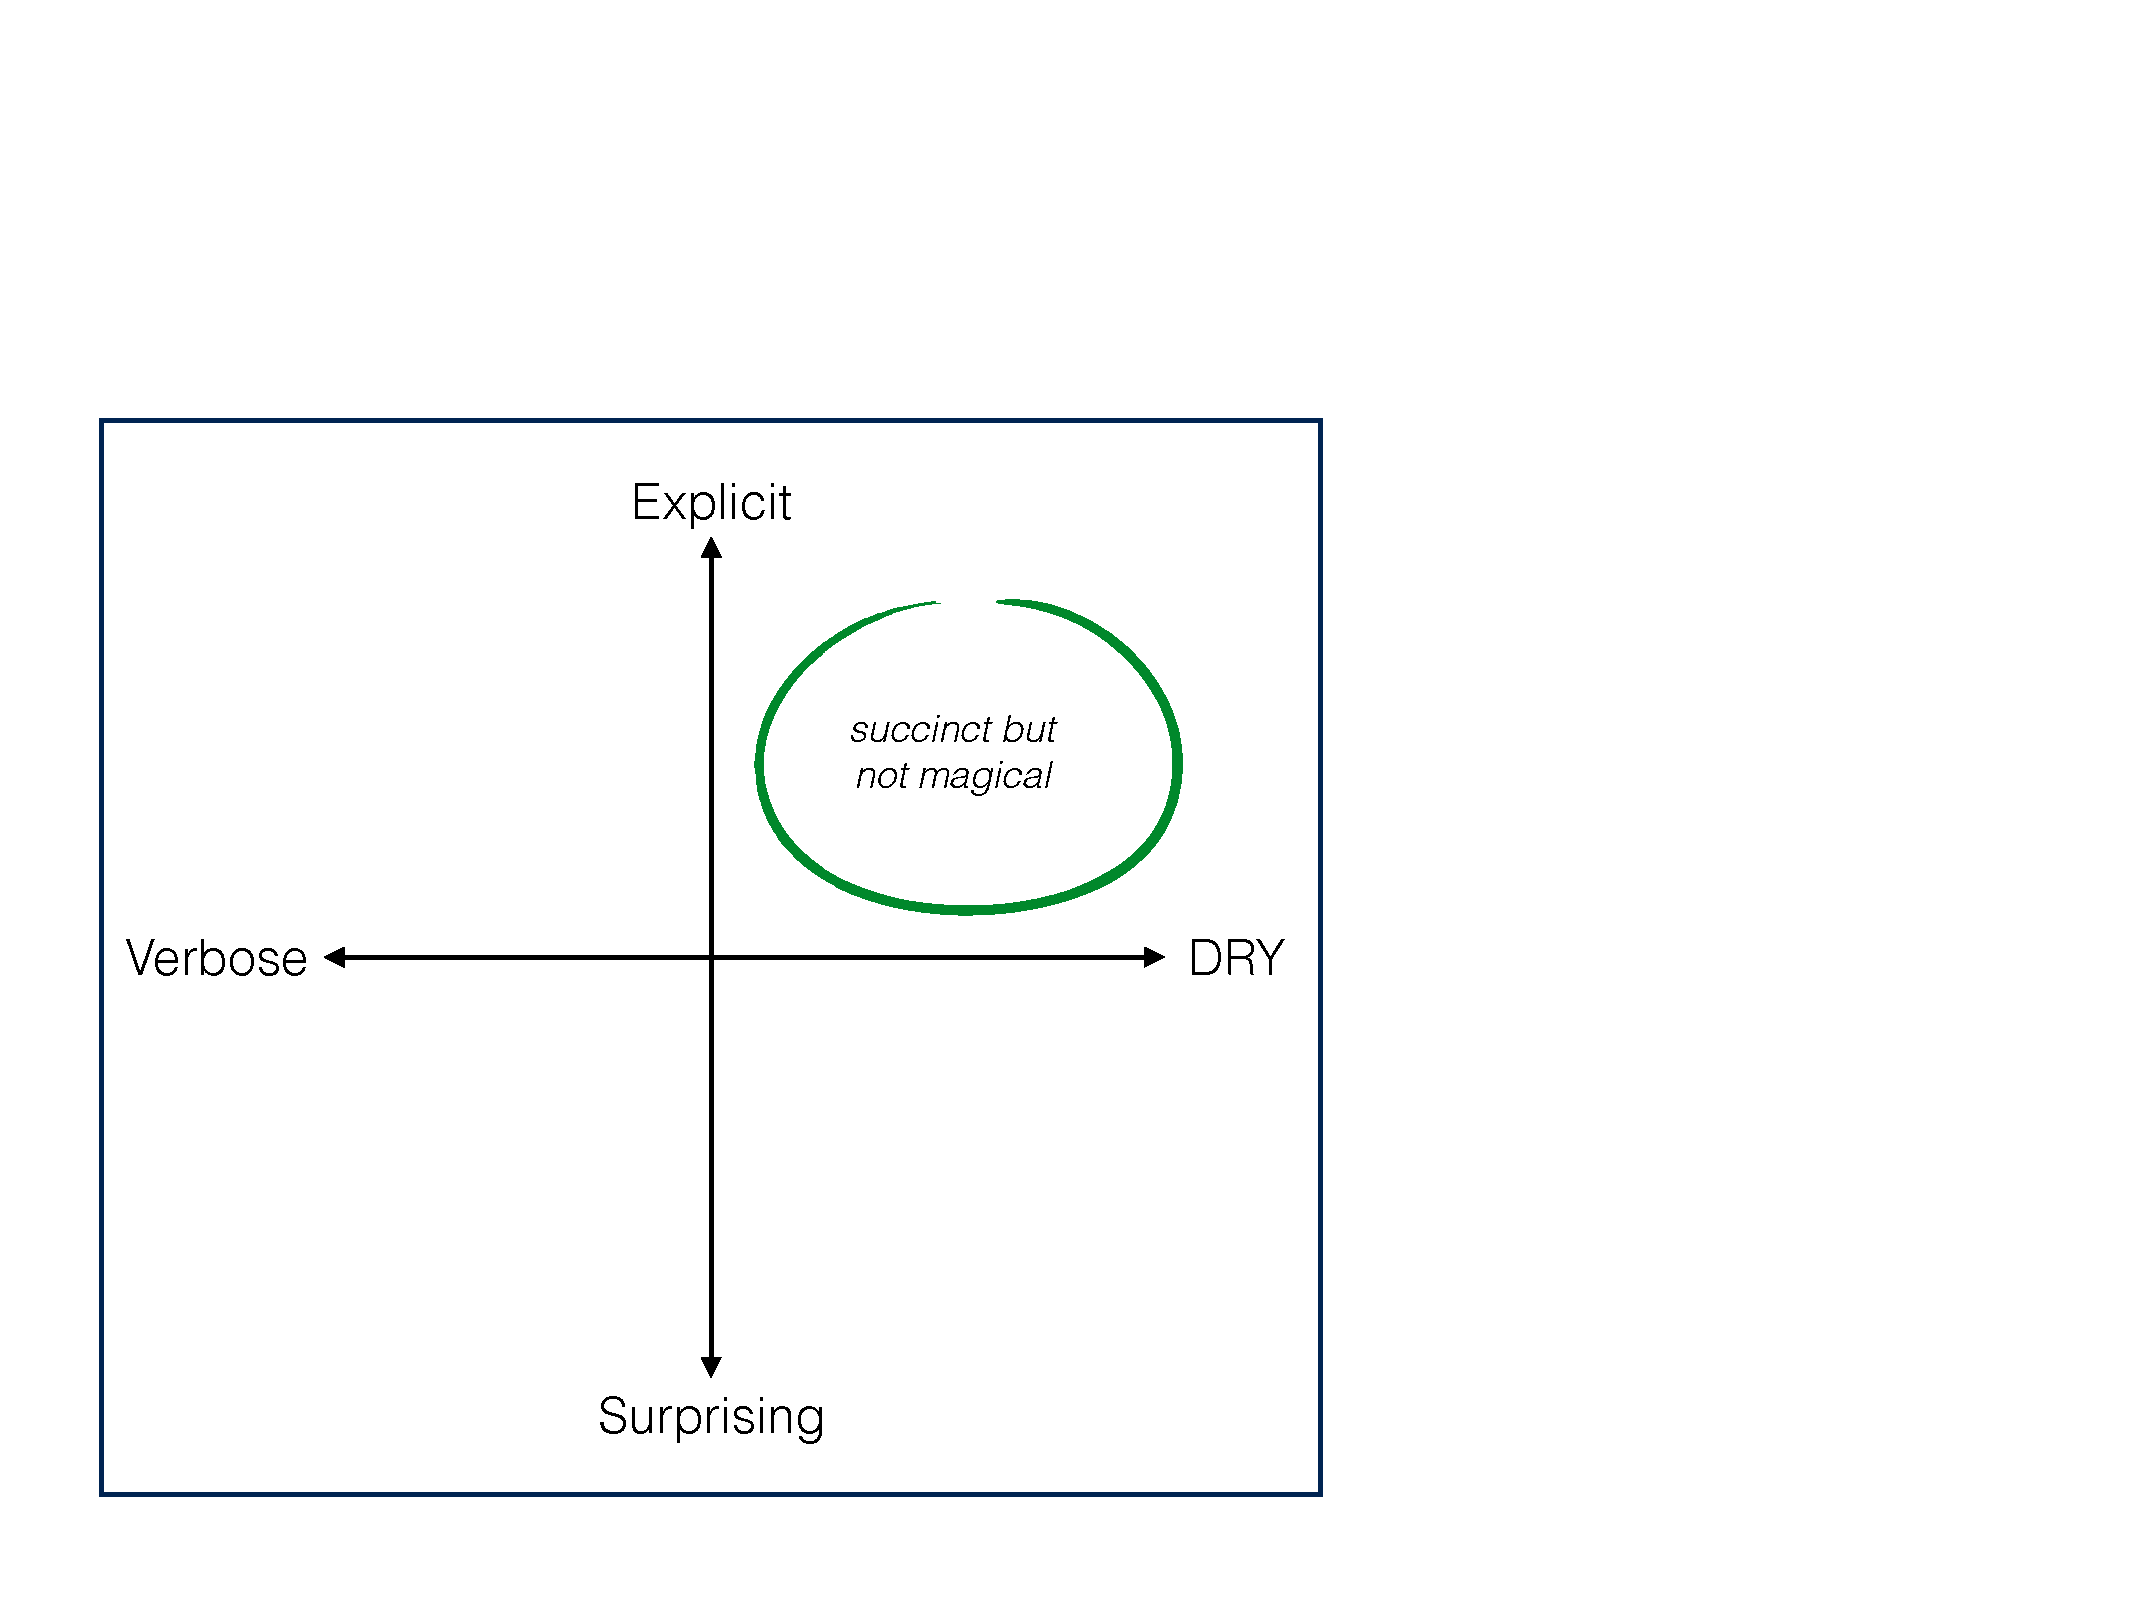
\includegraphics[width=.85\linewidth]{architecture-monitoring/coc}
\end{center}

These are the same two dimensions at play in the principle of
\href{https://en.wikipedia.org/wiki/Convention\_over\_configuration}{convention
over configuration}. The idea is that you'd like code to be consistently and
intuitively instrumented and observable with minimal developer effort, yet have
that instrumentation be flexible if you want or need to change it.
It's a goal that frameworks can help you achieve in some cases.

\section{Service Ownership}

Pick a service in your application. Who's responsible for running it in
production? Is it the same people who wrote it?

One of the core tenets of DevOps, which aligns well with microservices
architectures, is that those who write the code are responsible for making sure
it runs well in production too. This requires that they be
able to observe it in production. This is \emph{mandatory}. If the system isn't observable, full-lifecycle developer ownership is impossible, and DevOps breaks down and turns into silos.

This book isn't the place to dive deeply into the many valid reasons for this
viewpoint. But I do want to point out one of the main ways in which
silos hurt performance and reliability: the absence or interruption of feedback
loops. If a developer doesn't have to operate their systems in production, they
will not make those systems easy to operate. It's that simple. They won't know
what types of affordances those systems need; they won't know which log messages
are helpful or which are missing; and so on. Operability is a feature, and they
won't know how to make that feature work well.

If you agree with this argument, it's quite clear that every service running in
production needs to be highly observable.

\section{Common Observability Pitfalls}

In this section, I'll explore some of the observability problems I've seen, both in custom
software and in off-the-shelf systems. To begin with, here are some
topics that are mostly related to custom application code, but are also good
advice for anyone building server software for someone else to use:

\begin{description}

\item[Log Levels] There never seem to be enough logging levels to 
capture the desired granularity and relevance of a log message accurately. Is it INFO,
TRACE, or DEBUG? What if it's DEBUG but it's for a condition we should WARN
about? Is there really a linear hierarchy here? And if you're like most people,
you've seen at least once an extension of those types of standard logging levels
on top of a widely available logging system to add \emph{even more} custom
levels. I think there's a good argument that there should be only two
types of log messages: those useful for writing and debugging the code, and
those useful for operating it. Dave Cheney has a
\href{http://dave.cheney.net/2015/11/05/lets-talk-about-logging}{good blog post}
about this.

\item[Mixed Status and Configuration] Many systems don't distinguish between
status variables, which signal the system's state, and configuration variables,
which are inputs to the system's operation. For example, in both MySQL and
Redis, the commands to get system status will return mixtures of configuration
variables and status metrics. Such a metrics ``melting pot'' is a very common problem that usually
requires custom code or exception lists (blocklist/goodlist) to identify which
variables are what.

\item[Breaking Backwards Compatibility] If you change the meaning or dimensions
of a metric, ideally you should leave the old behavior unchanged and introduce a
replacement alongside it. Failure to do this causes a lot of work for other
systems. For example, in MySQL, the SHOW STATUS command was changed to include
connection-specific counters by default, with the old system-wide global
counters accessible via a different query syntax. This change was just a bad decision,
and it caused an enormous amount of grief. Likewise, the meaning of MySQL's
``Questions'' status variable was changed at one point, and the old behavior was
available in a new variable called ``Queries.'' Essentially, they
\href{http://dev.mysql.com/doc/refman/5.0/en/server-status-variables.html#statvar\_Questions}{renamed
a variable and then introduced a new, different variable with the same name as
the old one}. This change also caused a lot of confusion. Don't do this.

\item[Incomplete Visibility] Again the easiest example of this is in MySQL,
which has had a SHOW VARIABLES command for many years. Most, but not all, of the
server's commandline options had identically named variables visible in the
output of this command. But some were missing entirely, and others were present
but under names that didn't match.

\item[Missing Golden Signals] The list of golden signals for finding and diagnosing
performance issues isn't
that large: it's just CELT and USE. But you'd be surprised how many systems don't have any way
to inspect these key telemetry items,
because people who didn't know or prioritize observability built the systems (perhaps because they're not going to be the ones on-call when it breaks). For example,
PostgreSQL has a standard performance counter for transactions, but not for
statements, so if you want to know how many queries (statements) per second your
server is handling, you have to resort to much more complex alternatives. This
lack of a basic performance metric (throughput) is quite a serious oversight.

\end{description}

\section{Monitoring Tool Best Practices}

The previous section listed some of the biggest sins I've seen in custom and off-the-shelf
software applications, related to the ways they expose information about
themselves. Another category of pitfalls is mostly applicable to
\emph{monitoring software itself}:

\begin{description}

\item[Alert Severities] Similar to logging levels, not everything seems to fit
into Nagios severities (OK/WARN/CRIT/UNKNOWN), but less is probably more.
However, this is such a widely used standard that it's probably best to adhere
to it.

\item[Flap Mitigation] Flapping is a problem when a system's state alternates
between bad and good. Sometimes this is because it's hovering near a threshold
and crossing back and forth over it rapidly. Sometimes it's because a binary
condition is unstable, resolving and reappearing. Systems such as Nagios do a
crude form of detection of this condition, suppressing the repeated alarms that
would otherwise result. There are many possible ways to improve upon this, such
as having a reset threshold (alert when a metric is greater than X, but suppress
all further alerts until the metric drops back below a much lower value). But
the main thing is to have flap suppression at all.

\item[Alert Consolidation] Repeated or similar alerts from systems add a lot of burden
and activity without adding value. There are entire companies that specialize in
consolidating, aggregating, and deduplicating alerts. You can build duplicate
suppression into the source, however, through a variety
of mechanisms, including simplistic ones such as suppression periods after raising an
alert.

\item[Alert Cancellation] If an alert triggers a condition but there's no way to
cancel it automatically, you might suffer from the accumulation of
open conditions that are no longer relevant, and serve to create enough noise
that the value of the monitoring system rapidly decreases.

\item[Scheduled Maintenance] Removing or suppressing alerts about systems that
are known to be under maintenance is an indispensable feature at scale.

\end{description}

You'll notice that this list is aspirational. Few, if any, monitoring systems
or application code check all of these boxes. That's OK, but the more the
better.

\section{Inspecting Applications at Runtime}

Building always-on instrumentation into your application's architecture, so you
can connect to anything that's doing work and inspect it live, is a life saver.

This type of capability is often built in at some level, but the question is how
disruptive it is to use. For example, you can always use \texttt{gdb} to inspect
a process while it's live, but that'll freeze it for the duration. Some
programming languages, such as Erlang, are legendary for allowing nonintrusive
inspection and modification of running processes, but that's the exception, not
the norm.

At VividCortex, we use Go for our internal and external services, and we've
found it indispensable to use a few tools it offers, as well as adding our
own observability through frameworks and libraries we've built. You'll probably need to do
something similar, no matter what languages or frameworks you use. If you don't,
you'll wish you had.

Here are a few of the key techniques we've used:

\begin{description}

\item[Enabling Profiling] Go has a set of profiling libraries in the core
packages, which let engineers introspect a running binary non-disruptively.
These are extremely simple to include in a program (but not built in by
default), and expose themselves through HTTP endpoints. You can use these to
inspect CPU and memory profiles, among other things.

\item[Building a Processlist] Any system or application that handles requests needs a processlist. In fact, it's the foundation of workload observability. We've built a set of libraries that maintains
state for each service, showing what requests it's handling, what states they're
in, and enabling extra behaviors such as canceling them. These also expose an
HTTP interface, so they're easy to wrap into simple web applications and other
API clients.  The library is called \href{https://github.com/VividCortex/pm}{pm}
and is open source.

\end{description}

As a result, we're able to answer questions such as ``what requests are in
flight across all of our services?'' and take actions such as canceling a
request that is causing problems for others. You can
\href{https://www.vividcortex.com/blog/2014/11/06/inside-distributed-architecture/}{read more about this}
on our blog.

\section{Making Databases Observable}

The topic of measuring a database's workload (or really, any networked
service's workload) is important to consider separately, because it's so much
harder than monitoring something simple like CPUs or network interfaces.

To monitor such a service properly, as I mentioned previously, you need to
monitor the \emph{work} it is doing. If you're just monitoring status counters,
you're just looking at undifferentiated global vanity metrics that won't
reveal whether anyone is having any issues. You need deep drilldown into
the specific work the system is doing.

The problem is that such services typically have very high event rates, so
they're throwing off a lot of high-cardinality data if you capture and measure
it all. For example, there are many examples of server software handling
millions of queries per second (yes, even relational databases). If you record
all of these requests and all of the information about them---SQL, user, current
database, origin hostname, timestamp, latency, error codes, and so on---it's 
overwhelming. As a result, the best practice that's emerged over time is to
\emph{digest} away the variable portions of the SQL or other command text,
creating an abstracted statement without literal values. You use this to
group queries into categories or families. Then you generate metrics about the
categories, rather than recording the individual events.

Practically every usable monitoring tool for databases uses digests. This is how
MySQL Enterprise Monitor, pgBadger, VividCortex, pt-query-digest, and countless
others do it. Digesting results in a reduced volume of monitoring data that still
helps drill down into what's happening quite well. It's worth mentioning,
however, that even this reduced set of data is still typically thousands of
times larger than the usual system monitoring data you might be used to (CPU,
disk, network, memory, etc). It's a very large and challenging telemetry
workload.\footnote{As an aside, VividCortex doesn't discard individual events: it retains samples of them, so you can start your exploration with cheap, fast metrics and then drill into samples with their high-cardinality dimensions retained in full detail.}

What does this have to do with you, the application developer? Everything. The
way your application uses your database will either work well with query
analysis tools, or it'll cause a disaster.  Database monitoring systems
are built to categorize queries together, so try to make that easy by avoiding
spurious highly variable queries, and making your queries easily
digestible. This will not only reduce the burden on the monitoring system, but
it will also group related queries together correctly, so you don't miss queries
that are individually insignificant but are heavy hitters as a group.

You're trying to reduce entropy in the set of queries
your database is handling. Reducing diversity of workload can be good
for many reasons, but in this book, I'll continue to focus on the goal of
observability.

\section{Soothing Troubled Digestion}

Here's a list of best practices for making your app's
database workload easy for a monitoring system to digest and categorize.

\begin{description}

\item[Use Digestible Identifiers] Many highly partitioned systems will use
database names or filesystem directories to identify a partition. Query
digesting systems are typically designed to digest out easily identified numeric
portions of queries. If all of your queries include a fully-qualified database
name, for example, then ensure those are digestible, preferably with a numeric
identifier. As an example, most query monitoring systems will not digest the
following two statements into the same category of queries: \texttt{SELECT *
FROM acme.user} and \texttt{SELECT * FROM contoso.user}. You \emph{want}
those to be digested together if Acme and Contoso are customers, and you
have millions of customers. You should provide a partition directory service
that lets you write queries like \texttt{SELECT * FROM cust\_9184.user} instead.

\item[Avoid Variable-Number Repeated Parts] Some parts of queries can be
repeated in groups. For example, the number of parameters in an \texttt{IN()}
clause is arbitrary. Depending on how sophisticated the query digester is, that
might cause a problem. In PostgreSQL, the pg\_stat\_statements extension won't
digest the following statements together into the same category: 
\texttt{SELECT * FROM users WHERE id IN(1, 2, 3)} and
\texttt{SELECT * FROM users WHERE id IN(1, 2, 3, 4)}. In MySQL, the built-in
Performance Schema will digest those together.

Another example is a variable number of \texttt{UNION} clauses. I've seen
applications that chain together lots of different queries with \texttt{UNION},
and most query digesters aren't going to recognize those as the same query.
Similarly, if you have a statement of the form \texttt{INSERT INTO t
VALUES(...), (...), ...} where a variable number of parenthesized
\texttt{VALUES} clauses may appear, not all digest algorithms will handle that
well.

\item[Avoid Ordering Permutations] If you generate queries by iterating through
randomly ordered data structures, such as a hash (a.k.a. dictionary, map, set),
you can end up with random permutations of column names. At VividCortex, we had a
customer running a data load with a Ruby script that generated SQL statements in
this fashion. The destination table had more than ten columns. The number of
possible permutations of column orders is the factorial of the number of
columns, so this data load was creating many millions of apparently unrelated
metrics. This fragmented a primary source of load on the database, to the point it
was invisible to monitoring tools.

Another example we've seen is in BSON serialization libraries for sending
MongoDB queries. The fields in the BSON were ordered randomly. This one was
apparently not under developer control, so we had to build sorting into
VividCortex's query digesting algorithm for MongoDB.

\item[Make Queries Short] This is often beyond the developer's control, but many
query-generation tools will add spurious text, such as redundant AS clauses that
give every column a long name when it already has a perfectly good one.
Similarly, many of them will list all columns by name instead of using the
\texttt{*} syntax, or will select needless columns instead of only those the
application needs. The issue is that a lot of query metrics collection systems
have hard length limits, and this causes the query to be truncated. In a lot of
cases, all the useful information in the SQL is beyond the limit and all you get
is a list of column names, without the ability to see any table names, WHERE
clauses, or the like. (There are lots of other problems with autogenerated
queries, but these are the main ones that are relevant to monitoring systems.)

\item[Avoid System-Specific Magic] Sometimes people rely on specific features
such as injecting data into SQL comments, using particular syntax, and the like.
Although sometimes this can work well, in many cases it won't survive query
digesting algorithms, or it'll be removed for mysterious reasons
only in some circumstances. For example, by default the MySQL command-line
client tool will strip query comments before they're even sent to the server;
and depending on syntax and other circumstances some databases will remove such
comments during digesting. Sometimes you can work around this with
version-specific or database-specific comment syntax, but that's typically a
brittle system that will be prone to breaking in the future. If you must use
query comments, consider whether to add them at the beginning or end of the SQL,
because if you add them at the end they may be truncated and lost.

\end{description}

\section{Enabling Guerrilla Troubleshooting}

Some databases, especially those that don't have good built-in observability
(which is true of most open source databases, especially the newer ones), might
have to be instrumented through methods such as network traffic capture or log file
analysis. You can't always get everything you want from such sources of data.
The following best practices can help make your database workload more
explicitly observable.

\begin{description}

\item[Include Implicit Data In SQL]
If you're sniffing network traffic, anything \emph{stateful} about
a connection, such as the current database it's connected to, is only observable at
connection establishment. As a result, any given query that travels across the wire 
lacks implied information that had to have been captured at an earlier point
in time. Thus, if you're looking at a TCP dump, you might not be able to see
against which database a query executed. To counteract this, you can fully
qualify the query, e.g. \texttt{SELECT * FROM acme.user} rather than
\texttt{SELECT * FROM user}. As a bonus, this protects you against bugs when the
statement is issued with the wrong currently active database or search path!

The same principle applies to user-defined variables or parameters. If you're
examining a log and you see \texttt{SELECT * FROM acme.user WHERE id=\$1}, it's a
lot harder to troubleshoot and understand exactly what was happening. In some
cases, as a result, prepared statements and the like can hamper observability.

\item[Use Different Users For Different Purposes] It's a good idea to
avoid a single database user account that gets used for everything. Suppose you
have trouble with lots of open connections to your database, exceeding the
allowed connection limit. You log into the database and look at the connections.
There are thousands, all of them in an idle status, doing nothing. And all of
them are listed as the \texttt{app} username. You have a complex microservices
architecture with dozens of applications; which one is responsible for opening
all those connections? If you'd used different usernames per service, it would be
easier to tell.

\item[Use TCP, Not Unix Sockets] Most networked server software can use either
Unix sockets or TCP connections. MySQL, in particular, likes to default to a
Unix socket when connections come from localhost. Unfortunately, you can't sniff
a Unix socket the way you can sniff a TCP socket with tcpdump. To avoid this,
connect to 127.0.0.1 instead of localhost.

\item[Avoid Stored Code Such as Stored Procedures and Triggers] Most databases
offer poor visibility into what happens inside a stored procedure or its
equivalent. Even when possible, they're much more complicated to inspect 
than a straightforward statement.

\end{description}

\section{Observing Database-As-A-Service}

There are several special considerations for hosted databases, commonly called
DBaaS (database-as-a-service). The most popular is Amazon
RDS, which is available for a variety of database software such as MySQL,
Oracle, and PostgreSQL. But there are also providers such as
\href{http://compose.io}{Compose} and other cloud databases like Amazon
DynamoDB. 

In these scenarios, you get nearly full client-level access to a
database server, but no operating-system-level access at all. The database runs
on a box that you can't SSH to or otherwise manipulate except through tightly
defined avenues.

The appeal and ROI of renting a fully-managed database is undeniable.
The main tradeoff to consider is that in exchange, you get less observability and control
over the database. In particular, you're limited to the monitoring data that the
database provides, be that Performance Schema, pg\_stat\_statements, log files,
or the like.  You're also subject to the limitations of this
instrumentation.

You're also dependent on the hosting provider for giving you host-level metrics
about the underlying OS, such as CPU, IO, and network metrics. Those are
usually \emph{not} available through the database. What this means is that you
have to collect different types of metrics from different systems (e.g. query
performance metrics from a client connection to the database, CPU performance
metrics from Cloudwatch). And you then need to integrate and correlate those
together.

Are these limitations a problem? Not really. Just something to be aware of and
plan for explicitly. You don't want to be surprised after the fact.

\section{Conclusions}

Observability shouldn't be an afterthought, and \emph{observability is a feature},
just like security and usability. Databases, in particular, present
difficult observability challenges. In today's high-scale, distributed
application architectures, fine-grained observability is more important than ever.

There's a lot you can do as you architect your application to ensure it's 
easier to observe and monitor in production. The options range from basic hygiene to some very
subtle points, which are difficult to tackle later and much cheaper if you
address them up front.

In this book I've given you a quick end-to-end tour of what I've learned about
building highly observable applications, especially drawing from my team's
shared experience solving database performance problems for ourselves and
customers.  A few of the key takeaways are as follows:

\begin{itemize}
\item Measure what you should, not what you can.
\item Measure both externally customer-visible QoS and internal resource performance.
\item Learn from the mistakes others have made, so you can avoid repeating them.
\item Build the CELT+USE golden signals into your applications and make them easy to integrate with
monitoring systems.
\item Be extra sensitive to how you craft queries, lest you end up with a
database workload that no monitoring system can handle well.
\item Not every performance gain comes with good observability.
\item There's no free lunch, as usual.
\end{itemize}

Thanks to the talented engineering team at VividCortex for suggestions and
reviews. Mistakes and shortcomings are solely mine; many of the things you might
like about this book are their contributions.

\newpage

\begin{about}	% Build "About VividCortex"
VividCortex is SaaS database performance monitoring that significantly eases the pain of database performance at scale for the entire IT department. Unlike traditional monitoring, we measure
and analyze the system's work and resource consumption. This leads directly to better performance for IT as a whole, at reduced cost and effort.
\end{about}
\makeresources	% Build "Related Resources"
\end{document}
